\section{Describing data sets}\label{sec:describing-data-sets}

~\cite{ross_introduction_2009}

% frequency table {{{
\begin{table}[H]
  \centering
  \pgfplotstabletypeset[
    columns={
      Starting yearly salary,
      Frequency
    },
    col sep=comma,
    every head row/.style={before row=\toprule,after row=\midrule},
    every last row/.style={after row=\bottomrule},
  ]{src/starting-yearly-salaries.csv}
  \caption{Frequency table for starting yearly salaries}
  \label{tbl:starting-yearly-salaries}
\end{table}
% }}}

% line graph {{{
\begin{figure}[H]
  \centering
  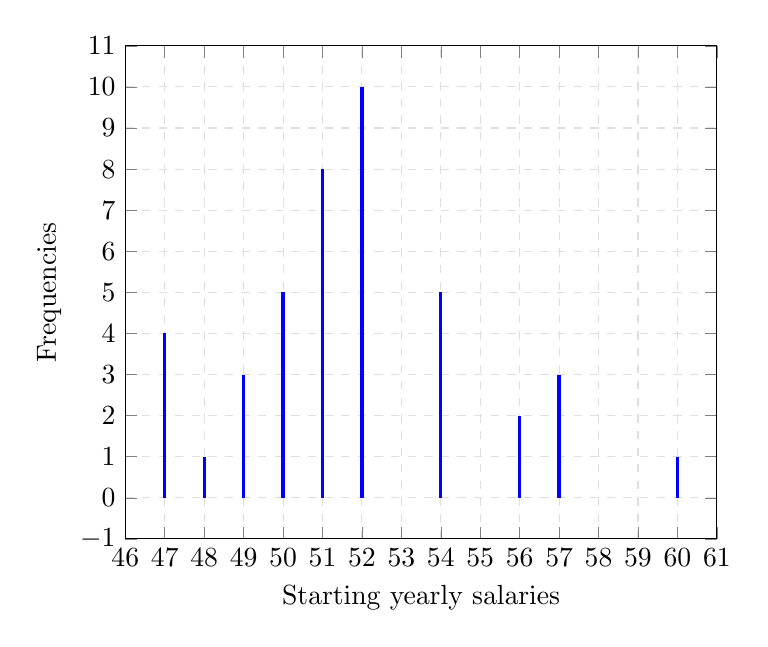
\begin{tikzpicture}
    \begin{axis}[
        grid             = both,
        major grid style = {dashed,gray!25},
        minor grid style = {dashed,gray!25},
        width            = 0.75\linewidth,
        xlabel           = {Starting yearly salaries},
        ylabel           = {Frequencies},
        xmin             = 46,
        xmax             = 61,
        ymin             = -1,
        ymax             = 11,
        xtick distance   = 1,
        ytick distance   = 1,
      ]
      \addplot[color=blue,very thick] coordinates { (47,0) (47,4) };
      \addplot[color=blue,very thick] coordinates { (48,0) (48,1) };
      \addplot[color=blue,very thick] coordinates { (49,0) (49,3) };
      \addplot[color=blue,very thick] coordinates { (50,0) (50,5) };
      \addplot[color=blue,very thick] coordinates { (51,0) (51,8) };
      \addplot[color=blue,very thick] coordinates { (52,0) (52,10)};
      \addplot[color=blue,very thick] coordinates { (53,0) (53,0) };
      \addplot[color=blue,very thick] coordinates { (54,0) (54,5) };
      \addplot[color=blue,very thick] coordinates { (56,0) (56,2) };
      \addplot[color=blue,very thick] coordinates { (57,0) (57,3) };
      \addplot[color=blue,very thick] coordinates { (60,0) (60,1) };
    \end{axis}
  \end{tikzpicture}
  \caption{Line graph for starting salary data}
  \label{fig:line-graph-frequencies-yearly-salaries}
\end{figure}
% }}}

% bar graph {{{
\begin{figure}[H]
  \centering
  \begin{tikzpicture}
    \begin{axis}[
        grid             = both,
        major grid style = {dashed,gray!25},
        minor grid style = {dashed,gray!25},
        width            = 0.75\linewidth,
        xlabel           = {Starting yearly salaries},
        ylabel           = {Frequencies},
        xmin             = 46,
        xmax             = 61,
        ymin             = -1,
        ymax             = 11,
        xtick distance   = 1,
        ytick distance   = 1,
        ybar,
      ]
      \addplot
      table[
        x       = Starting yearly salary,
        y       = Frequency,
        col sep = comma,
      ]{src/starting-yearly-salaries.csv};
    \end{axis}
  \end{tikzpicture}
  \caption{Bar graph for starting salary data}
  \label{fig:bar-frequencies-yearly-salaries}
\end{figure}
% }}}

% frequency polygon {{{
\begin{figure}[H]
  \centering
  \begin{tikzpicture}
    \begin{axis}[
        grid             = both,
        major grid style = {dashed,gray!25},
        minor grid style = {dashed,gray!25},
        width            = 0.75\linewidth,
        xlabel           = {Starting yearly salaries},
        ylabel           = {Frequencies},
        xmin             = 46,
        xmax             = 61,
        ymin             = -1,
        ymax             = 11,
        xtick distance   = 1,
        ytick distance   = 1,
      ]
      \addplot
      table[
        x       = Starting yearly salary,
        y       = Frequency,
        col sep = comma,
      ]{src/starting-yearly-salaries.csv};
    \end{axis}
  \end{tikzpicture}
  \caption{Frequency polygon for starting salary data}
  \label{fig:plot-frequencies-yearly-salaries}
\end{figure}
% }}}

\begin{example}
  The following data relate to the different types of cancers affecting the 200
  most recent patients to enroll at a clinic specializing in cancer. These data
  are represented in the frequency table~\ref{tbl:different-types-of-cancers}
  and also in the pie chart~\ref{fig:pie-chart-different-types-of-cancers}.
  % frequency table {{{
  \begin{table}[H]
    \centering
    \begin{tabular}{lll}
      \toprule
      Type of Cancer & Number of New Cases & Relative Frequency \\
      \midrule
      Lung           & 42                  & .21  \\
      Breast         & 50                  & .25  \\
      Colon          & 32                  & .16  \\
      Prostate       & 55                  & .275 \\
      Melanoma       & 9                   & .045 \\
      Bladder        & 12                  & .06  \\
      \bottomrule
    \end{tabular}
    \caption{Frequency table for different types of cancers}
    \label{tbl:different-types-of-cancers}
  \end{table}
  % }}}
  % pie chart {{{
  \begin{figure}[H]
    \centering
    \begin{tikzpicture}
      \pie[sum=200]{42/Lung,50/Breast,32/Colon,55/Prostate,9/Melanoma,12/Bladder}
    \end{tikzpicture}
    \caption{Pie chart for different types of cancers}
    \label{fig:pie-chart-different-types-of-cancers}
  \end{figure}
  % }}}
\end{example}

\subsection{Grouped Data}\label{ssec:grouped-data}

% a very long table {{{
\begin{table}[H]
  \centering
  \begin{tabular}{rrrrrrrrrr}
    1.067 & 919   & 1.196 & 785   & 1.126 & 936   & 918   & 1.156 & 920   & 948   \\
    855   & 1.092 & 1.162 & 1.170 & 929   & 950   & 905   & 972   & 1.035 & 1.045 \\
    1.157 & 1.195 & 1.195 & 1.340 & 1.122 & 938   & 970   & 1.237 & 956   & 1.102 \\
    1.022 & 978   & 832   & 1.009 & 1.157 & 1.151 & 1.009 & 765   & 958   & 902   \\
    923   & 1.333 & 811   & 1.217 & 1.085 & 896   & 958   & 1.311 & 1.037 & 702   \\
    521   & 933   & 928   & 1.153 & 946   & 858   & 1.071 & 1.069 & 830   & 1.063 \\
    930   & 807   & 954   & 1.063 & 1.002 & 909   & 1.077 & 1.021 & 1.062 & 1.157 \\
    999   & 932   & 1.035 & 944   & 1.049 & 940   & 1.122 & 1.115 & 833   & 1.320 \\
    901   & 1.324 & 818   & 1.250 & 1.203 & 1.078 & 890   & 1.303 & 1.011 & 1.102 \\
    996   & 780   & 900   & 1.106 & 704   & 621   & 854   & 1.178 & 1.138 & 951   \\
    1.187 & 1.067 & 1.118 & 1.037 & 958   & 760   & 1.101 & 949   & 992   & 966   \\
    824   & 653   & 980   & 935   & 878   & 934   & 910   & 1.058 & 730   & 980   \\
    844   & 814   & 1.103 & 1.000 & 788   & 1.143 & 935   & 1.069 & 1.170 & 1.067 \\
    1.037 & 1.151 & 863   & 990   & 1.035 & 1.112 & 931   & 970   & 932   & 904   \\
    1.026 & 1.147 & 883   & 867   & 990   & 1.258 & 1.192 & 922   & 1.150 & 1.091 \\
    1.039 & 1.083 & 1.040 & 1.289 & 699   & 1.083 & 880   & 1.029 & 658   & 912   \\
    1.023 & 984   & 856   & 924   & 801   & 1.122 & 1.292 & 1.116 & 880   & 1.173 \\
    1.134 & 932   & 938   & 1.078 & 1.180 & 1.106 & 1.184 & 954   & 824   & 529   \\
    998   & 996   & 1.133 & 765   & 775   & 1.105 & 1.081 & 1.171 & 705   & 1.425 \\
    610   & 916   & 1.001 & 895   & 709   & 860   & 1.110 & 1.149 & 972   & 1.002 \\
  \end{tabular}
  \caption{Life in hours of 200 incandescent lamps}
  \label{tbl:file-in-hours-of-200-incandescent-lamps}
\end{table}
% }}}
% class frequency table {{{
\begin{table}[H]
  \centering
  \begin{tabular}{rrrr}
    % \toprule
    % Class Interval & Number of Data Values in the Interval \\
    % \midule
    500  & -- & 600  & 2  \\
    600  & -- & 700  & 5  \\
    700  & -- & 800  & 12 \\
    800  & -- & 900  & 25 \\
    900  & -- & 1000 & 58 \\
    1000 & -- & 1100 & 41 \\
    1100 & -- & 1200 & 43 \\
    1200 & -- & 1300 & 7  \\
    1300 & -- & 1400 & 6  \\
    1400 & -- & 1500 & 1  \\
    \bottomrule
  \end{tabular}
  \caption{A class frequency table}
  \label{tbl:class-frequency-table}
\end{table}
% }}}

